\documentclass[11pt, xcolor=dvipsnames,twocolumn]{article}
\usepackage{graphicx}


\usepackage{geometry}
 \geometry{
 a4paper,
 total={170mm,240mm},
 left=20mm,
 top=25mm,
 }


% \title{STC Project Proposal \\ Analysis of magnetic field oscillation in adiabatic slower}

% \author{Yu Lu id Dept. of Physics\\ Xingyao Wang id Dept. of \\ Nitish Mittal id Dept. of}
% \date{\today}

\begin{document}
\begingroup  
  \centering
  \LARGE STC Project Proposal\\[0.5em]
  \large Yu Lu (id:superlu) \\  Nitish Mittal (id:nm23456)\\Xingyao Wang (id:xw2695)\\[0.5em]\par 
  \large Oct. 27, 2016\\
  \endgroup
  
%\maketitle
\section{Introduction}
Adiabatic slower is a facility that consist of hundreds of overlapping Anti-Helmholtz coils, which is used to slow atoms from $\sim 500 m/s$ down to $\sim 0 m/s$ to create ultra bright cold atom source in atomic physics. It is realized by activiting apatially overlapped magnetic traps with a overlapping time sequence, thus create an effective co-moving trap to slow down atoms. While its performance has been highly evaluated in the experiment\footnote{E. Narevicious, et. al., New Journal of Physics 13 (2011)}, the optimization hasn't been well discussed in any published articles. One of the key feature is the magnetic field oscillation during the trasition of traps, which is related to the lose rate, temperature, density of atoms being slowd. Here we propose a simulation approach to this problem, we will discuss the oscillation of magnetic field in adiabatic slower under different conditions, and try to find the optimized operating parameters for a given adiabatic slower setup.

\section{Description}
Anti-Helmholtz coil is a pair of coils with current propogating at opposite direction. Some atoms at special quantum states tend to stay at the magnetic field minimum to lower their energy, as shown in \ref{fig1}.\\ \begin{figure}[h!] 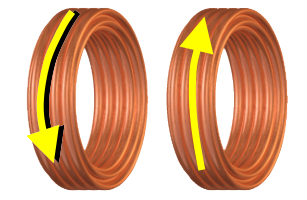
\includegraphics[width = 0.2\textwidth, height= 0.15\textwidth]{antiHelmholtz} 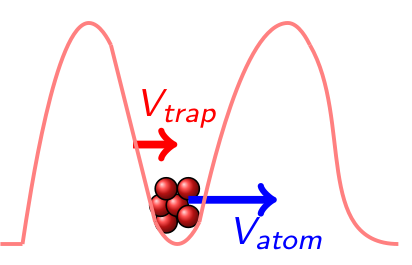
\includegraphics[width = 0.2\textwidth, height= 0.15\textwidth]{trap} \caption{(A) Anti-Helmholtz coil. (B) Atoms in the magnetic trap} \label{fig1} \end{figure} The trap basically provide a confinement of atoms, and can be treated as a 'carrier'. If we can control the moving speed of this 'carrier', then we can control the atoms confined by it. To realize this, a series of this kind of traps are activated in an overlapping sequence, both in real space and in time space, thus an effective moving trap can be created, as shown in \ref{fig2}. Usually these trap are switched on and off with hundreds of microseconds.\\\begin{figure}[h!]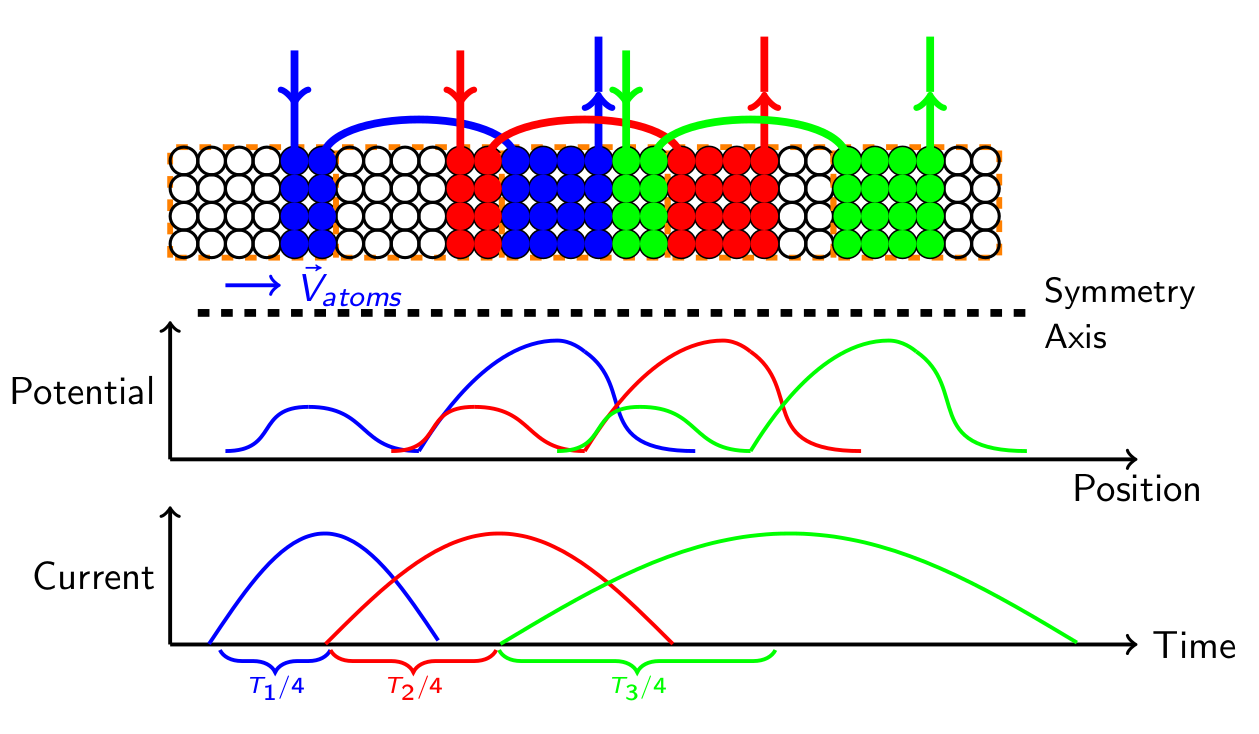
\includegraphics[width = 0.5\textwidth, height=0.3\textwidth]{switching} \caption{Schematic for generating co-moving magnetic trap} \label{fig2}\end{figure}

\section{Plan}
Publised article has shown that the total magnetic field minimum is oscillating during the trasition from one anti-helmholtz coils to the next ones, but detailed study hasn't been done. The transition oscillation is depend on: \begin{itemize} \item Overlapping of traps in space. \item Overlapping of current sequence in time. \item Current pulse shape (sin, triangle, etc.). \item  Anti-Helmholtz coil geometry. \end{itemize}

We will use C++ to simulate the transition of magnetic trap, cover the discussion of influence of one or few factors listed above. By programming, we will give a set of optimized operating parameters to minimize the oscillation of magnetic field during the trasition, provide a guidline to the experiment in cold atom physics.
\end{document}

